\chapter{ The Problem of Pattern Prediction and the Proposed Approach }

\label{chapter:system}

\par In this chapter, we introduce our proposed approach for pattern prediction over multiple input event streams. We start by defining the problem that we address in this thesis, which is divided into two parts: the formal definition of the pattern prediction over an individual event stream, then it is extended to the case of multiple streams. We present the used base model for event pattern prediction, and our proposed approach to leverage the distributed online protocol to enable knowledge sharing between prediction models over multiple event streams. Furthermore, we provide an analysis of the theoretical aspects of the proposed approach.

\par We follow the general notation and terminology of \cite{agrawal2008efficient,schultz2009distributed,luckham2008power,alevizos2015complex,zhou_pattern_2015,kamp2014communication} to formalize the problem we tackle and our solution approach.


\section{Pattern Prediction over a Single Event Stream}


\par In this section, we define the first part of the problem that we tackle in this thesis, by defining the problem of pattern prediction over a single event stream. We also give an introduction of the base prediction model, which is built based on the event forecasting with pattern Markov chains method \cite{alevizos2017event}.


\subsection{Basic Problem Formulation}

We first define the input event and the stream of events as follows:  
\begin{definition}
	Each event is defined as a tuple of attributes denoted by $e_i$, where 
	$e_i = (id,type,\tau,a_1,a_2,\ldots,a_n)$, $type\in\Sigma$ is the event type attribute that takes a value from a set of finite event types/symbols $\Sigma$, $\tau\in\R$ represents the time when the event tuple was created,  the  $a_1,a_2,...,a_n$ are spatial or other contextual features (e.g., speed); these features vary from one application domain to another. The attribute $id\in\N$ is a unique identifier that connects the event tuple to an associated domain object.
\end{definition}

\begin{definition}
A stream $s=\langle e_1,e_3,...,e_t,...\rangle$  is a time-ordered sequence of events.
\end{definition}


\par A user-defined pattern $\mathcal{P}$ is given in the form of a regular expression over a set of event types $\Sigma$ (i.e., alphabet). Let a word over $\Sigma$ be a sequence of event types, and the set of words over $\Sigma$ be a language $L$. Then $L(\mathcal{P})$ is the regular language defined by the regular expression ($\mathcal{P}$) \cite{hopcroft2006automata,nuel_pattern_2008,alevizos2017event},  where a regular expression is an event type $\in$ $\Sigma$, or defined using the following operators over regular expressions:
 
\begin{itemize}[noitemsep]
	\item \textit{sequence} that represents a concatenation of two regular expressions languages 
	\item \textit{disjunction} i.e., union, which is the language that its words belong to one of the languages of the two regular expressions 
	\item \textit{iteration} operation to define the set of all possible concatenation over a regular expression
\end{itemize}

More formally, a pattern is given through the following grammar:
\begin{definition}
$\mathcal{P} := E\ |\ \mathcal{P}_{1} ; \mathcal{P}_{2}\ | \mathcal{P}_{1} \vee \mathcal{P}_{2}\ |\ \mathcal{P}_{1}^{*}  $, where $E \in \Sigma$ is a constant event type. $;$ stands for sequence, $\vee$ for disjunction and $*$ for $\mathit{Kleene}-*$.
The pattern $\mathcal{P} := E$ is matched by reading an event $e_i$ iff $e_{i}.type = E$.
The other cases are matched as in standard automata theory.
\end{definition}


The $\mathcal{P}$ (regular expression) is encoded by a deterministic finite automaton (DFA). We define the DFA as following: 

\begin{definition}[\cite{hopcroft2006automata}]
	$(\Sigma,Q,s,F,\delta)$ is a deterministic finite automaton (DFA)  where  $\Sigma$ a finite alphabet of event types, and $Q$ is a finite set of states, $s \in Q$ a start state and $F \subset Q$ represents all final states. $\delta: Q \times \Sigma \rightarrow Q$ is a transition function from a state to another state given an input event type, which is defined as recursive function $\delta(q,e_{1}e_{2}\ldots e_{d})=\delta(\delta(q,e_{1}e_{2}...e_{d-1}),e_{d})$. If $\delta(s,w) \in F$ of a word $w=e_{1}e_{2}\ldots e_{d} \in \Sigma^{*}$, then the word $w$ is said to be accepted by the DFA. In addition,  $\delta(q)^{-m}$ is the set of words of size $m$ defined as $\{w \in \Sigma^{m} \mid \exists q \in Q,\ \delta(p,w)=q \}$
\end{definition}


\par The problem setting can be summarized as follows: given a stream $s$ of low-level events and a pattern $\mathcal{P}$, 
the goal is to estimate at each new event arrival the number of future events
that we will need to wait for until the pattern is completed (full match).

\subsection{Base Prediction Model}
\label{sec:Event-Forecasting-PMC}

\par In this thesis, we use the event forecasting with pattern Markov chains method \cite{alevizos2017event} to construct a pattern prediction model over an event stream. Next, we describe the details of this approach. We first provide an overview of the Patten Markov Chain framework \cite{nuel_pattern_2008}. Then, we describe how this framework is used to build a pattern prediction model \cite{alevizos2017event}.  


\subsubsection*{Pattern Markov Chain (PMC)}

~\citet{alevizos2017event} proposed to employ the Pattern Markov Chain (PMC) \cite{nuel_pattern_2008} to build an online prediction model associated with a pattern over an event stream. The algorithm of constructing a PMC associated with a pattern $\mathcal{P}$ over a stream of events $s$ consists of the following steps:

\begin{itemize}[noitemsep]
	\item Build a DFA that accepts the regular expression $\Sigma^{*};\mathcal{P}$. Firstly, the regular expression $\Sigma^{*};\mathcal{P}$ is converted to non-deterministic finite automaton (NFA), then an equivalent DFA of the constructed NFA is computed using the subset construction \cite{hopcroft2006automata,alevizos2017event}. And the events stream $s$ is considered as the input word of the DFA. 

\par Furthermore, if $\forall q \in Q$ of a DFA the all $\delta(q)^{-m}$ are sets of cardinality 1, then the DFA is called \textit{m-unambiguous}. ~\citet{nuel_pattern_2008} proposed a procedure to transform any DFA to an \textit{m-unambiguous} DFA, which is achieved by incrementally duplicate all states have m-ambiguity (i.e., $\vert\delta(q)^{-m}\vert > 1$).   Figure ~\ref{fig:dfa_adc} shows an associated DFA of a sequential pattern $\mathcal{P}=a ; d ; c$ over an alphabet $\Sigma=\{a,b,c,d\}$. 


%\begin{figure}[!ht]
%\begin{centering}
%
%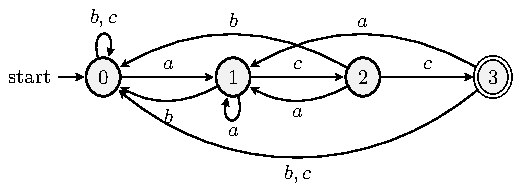
\includegraphics[width=0.35\textwidth]{./chapters/figures/forecasting/dfasr.pdf}
%\label{fig:dfa_adc}
%
%\hfill
%
%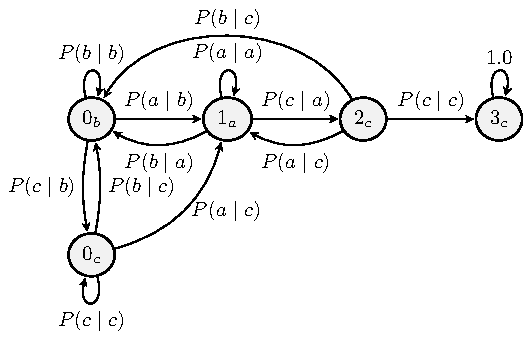
\includegraphics[width=0.35\textwidth]{./chapters/figures/forecasting/pmcr1.pdf}
%\label{fig:mc_adc}
%
%%\hfill
%\caption{DFA and PMC for $\mathcal{P}=a ; c ; c$,  $\Sigma=\{a,b,c\}$, and order $m=1$.}
%\label{fig:dfa_mc}
%\end{centering}
%\end{figure}

\begin{figure}[!h]
	\begin{centering}
		
			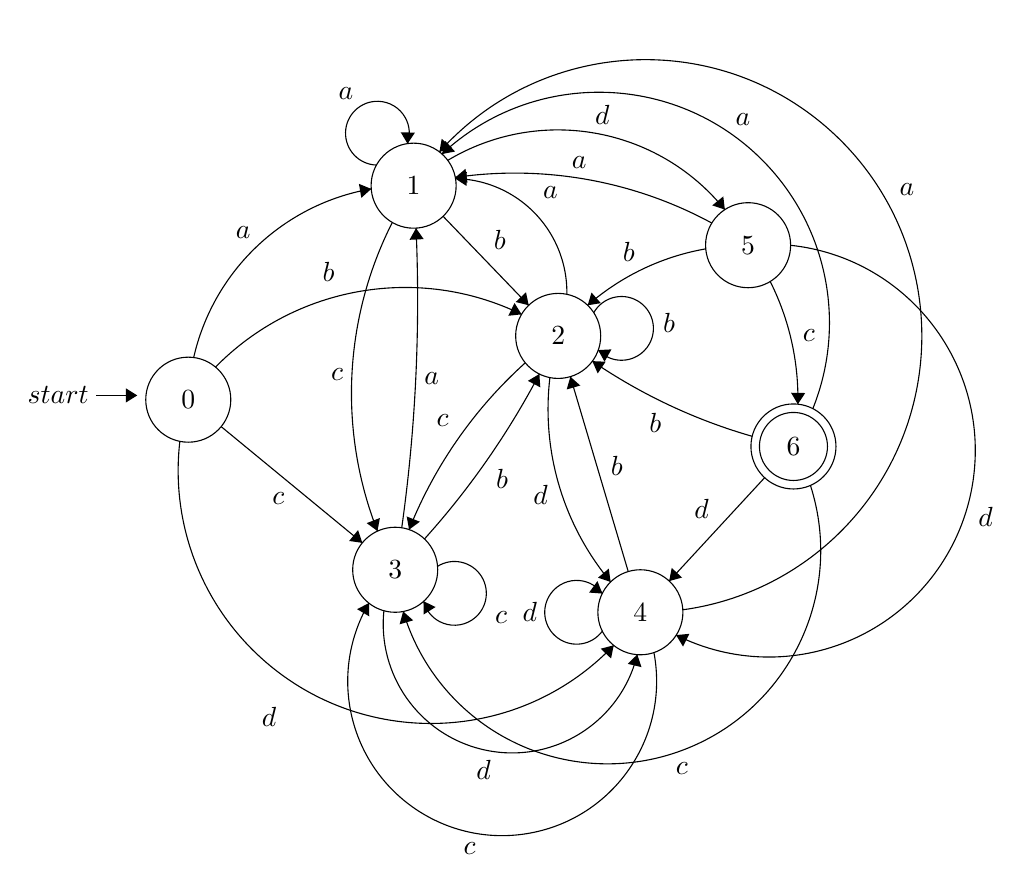
\begin{tikzpicture}[scale=0.18]
			\tikzstyle{every node}+=[fill=white,inner sep=0pt]
			\draw [black] (-2.6,-23.8) -- (0.3,-23.8);
			\draw (-3.1,-23.8) node [left] {$start$};
			\fill [black] (0.3,-23.8) -- (-0.5,-23.3) -- (-0.5,-24.3);
			\draw [black] (3.9,-24.1) circle (3);
			\draw (3.9,-24.1) node {$0$};
			\draw [black] (19.8,-9) circle (3);
			\draw (19.8,-9) node {$1$};
			\draw [black] (30,-19.6) circle (3);
			\draw (30,-19.6) node {$2$};
			\draw [black] (18.5,-36.1) circle (3);
			\draw (18.5,-36.1) node {$3$};
			\draw [black] (35.8,-39.1) circle (3);
			\draw (35.8,-39.1) node {$4$};
			\draw [black] (43.4,-13.2) circle (3);
			\draw (43.4,-13.2) node {$5$};
			\draw [black] (46.6,-27.4) circle (3);
			\draw (46.6,-27.4) node {$6$};
			\draw [black] (46.6,-27.4) circle (2.4);
			\draw [black] (33.919,-41.432) arc (-43.70358:-186.66407:17.839);
			\fill [black] (33.92,-41.43) -- (33,-41.67) -- (33.73,-42.36);
			\draw (11.22,-45.77) node [below] {$d\mbox{ }\mbox{ }\mbox{ }\mbox{ }\mbox{ }$};
			\draw [black] (6.22,-26) -- (16.18,-34.2);
			\fill [black] (16.18,-34.2) -- (15.88,-33.3) -- (15.25,-34.07);
			\draw (10.25,-30.59) node [below] {$c$};
			\draw [black] (5.821,-21.8) arc (135.53989:64.02493:18.753);
			\fill [black] (27.42,-18.08) -- (26.92,-17.28) -- (26.48,-18.18);
			\draw (15.1,-15.77) node [above] {$b\mbox{ }\mbox{ }\mbox{ }\mbox{ }$};
			\draw [black] (4.28,-21.129) arc (167.20329:99.84016:15.584);
			\fill [black] (16.81,-9.23) -- (15.94,-8.87) -- (16.11,-9.86);
			\draw (7.78,-12.8) node [above] {$a$};
			\draw [black] (17.19,-7.545) arc (268.59189:-19.40811:2.25);
			\draw (15.02,-2.94) node [above] {$a$};
			\fill [black] (19.37,-6.04) -- (19.89,-5.26) -- (18.89,-5.23);
			\draw [black] (32.505,-17.971) arc (150.77527:-137.22473:2.25);
			\draw (37.37,-18.68) node [right] {$b$};
			\fill [black] (32.82,-20.6) -- (33.27,-21.42) -- (33.76,-20.55);
			\draw [black] (21.479,-35.863) arc (122.28011:-165.71989:2.25);
			\draw (25.52,-39.48) node [right] {$c$};
			\fill [black] (20.5,-38.32) -- (20.5,-39.26) -- (21.35,-38.73);
			\draw [black] (17.251,-33.374) arc (-158.59999:-206.89281:26.653);
			\fill [black] (17.25,-33.37) -- (17.42,-32.45) -- (16.49,-32.81);
			\draw (14.87,-22.35) node [left] {$\mbox{ }\mbox{ }\mbox{ }\mbox{ }\mbox{ }\mbox{ }\mbox{ }\mbox{ }c$};
			\draw [black] (22.205,-7.215) arc (120.91152:38.90637:15.136);
			\fill [black] (41.76,-10.69) -- (41.65,-9.76) -- (40.87,-10.39);
			\draw (33.11,-4.71) node [above] {$d$};
			\draw [black] (22.741,-8.501) arc (88.91183:-1.11524:8.025);
			\fill [black] (22.74,-8.5) -- (23.53,-9.02) -- (23.55,-8.02);
			\draw (28.9,-9.49) node [right] {$a$};
			\draw [black] (19.478,-33.265) arc (158.24167:132.00767:31.599);
			\fill [black] (19.48,-33.27) -- (20.24,-32.71) -- (19.31,-32.34);
			\draw (22.31,-25.55) node [left] {$c$};
			\draw [black] (33.704,-36.958) arc (-140.13045:-186.74081:19.012);
			\fill [black] (33.7,-36.96) -- (33.57,-36.02) -- (32.81,-36.66);
			\draw (29.3,-30.79) node [left] {$\mbox{ }\mbox{ }d$};
			\draw [black] (35.581,-42.078) arc (-13.66199:-186.01371:9.092);
			\fill [black] (35.58,-42.08) -- (34.91,-42.74) -- (35.88,-42.97);
			\draw (24.73,-49.48) node [below] {$d$};
			\draw [black] (19.971,-11.995) arc (2.52337:-8.01617:115.218);
			\fill [black] (19.97,-12) -- (19.51,-12.82) -- (20.51,-12.77);
			\draw (20.52,-22.61) node [right] {$a$};
			\draw [black] (21.88,-11.16) -- (27.92,-17.44);
			\fill [black] (27.92,-17.44) -- (27.73,-16.52) -- (27,-17.21);
			\draw (25.43,-12.83) node [right] {$b$};
			\draw [black] (28.674,-22.291) arc (-27.74002:-42.01064:57.083);
			\fill [black] (28.67,-22.29) -- (27.86,-22.77) -- (28.74,-23.23);
			\draw (25.58,-29.72) node [right] {$b$};
			\draw [black] (22.741,-8.416) arc (98.28712:61.53076:29.155);
			\fill [black] (22.74,-8.42) -- (23.6,-8.8) -- (23.46,-7.81);
			\draw (33.11,-7.86) node [above] {$a\mbox{ }\mbox{ }\mbox{ }\mbox{ }\mbox{ }$};
			\draw [black] (32.077,-17.44) arc (131.12228:99.93712:17.189);
			\fill [black] (32.08,-17.44) -- (33.01,-17.29) -- (32.35,-16.54);
			\draw (34.99,-14.37) node [above] {$b$};
			\draw [black] (44.959,-15.759) arc (26.66951:-1.27035:18.386);
			\fill [black] (46.91,-24.42) -- (47.43,-23.63) -- (46.43,-23.61);
			\draw (47.22,-19.58) node [right] {$c$};
			\draw [black] (46.395,-13.207) arc (83.9582:-116.6654:14.567);
			\fill [black] (38.32,-40.71) -- (38.81,-41.52) -- (39.26,-40.62);
			\draw (59.61,-32.38) node [right] {$d$};
			\draw [black] (44.57,-29.6) -- (37.83,-36.9);
			\fill [black] (37.83,-36.9) -- (38.74,-36.65) -- (38.01,-35.97);
			\draw (40.67,-31.79) node [left] {$d$};
			\draw [black] (43.687,-26.684) arc (-106.00985:-124.32589:39.144);
			\fill [black] (32.41,-21.38) -- (32.79,-22.25) -- (33.35,-21.42);
			\draw (36.85,-24.99) node [below] {$b$};
			\draw [black] (47.797,-30.145) arc (17.84688:-163.44093:15.041);
			\fill [black] (19.06,-39.04) -- (18.81,-39.95) -- (19.77,-39.67);
			\draw (38.73,-49.67) node [below] {$c$};
			\draw [black] (21.796,-6.766) arc (132.94565:-21.89007:16.264);
			\fill [black] (21.8,-6.77) -- (22.72,-6.59) -- (22.04,-5.85);
			\draw (43.03,-4.76) node [above] {$a$};
			\draw [black] (33.12,-40.423) arc (324:36:2.25);
			\draw (28.55,-39.1) node [left] {$d$};
			\fill [black] (33.12,-37.78) -- (32.77,-36.9) -- (32.18,-37.71);
			\draw [black] (36.754,-41.934) arc (10.72301:-210.39871:10.898);
			\fill [black] (16.65,-38.45) -- (15.81,-38.88) -- (16.67,-39.39);
			\draw (23.75,-55.29) node [below] {$c$};
			\draw [black] (34.94,-36.22) -- (30.86,-22.48);
			\fill [black] (30.86,-22.48) -- (30.6,-23.38) -- (31.56,-23.1);
			\draw (33.67,-28.75) node [right] {$b$};
			\draw [black] (21.619,-6.618) arc (138.23159:-82.24481:19.498);
			\fill [black] (21.62,-6.62) -- (22.52,-6.35) -- (21.78,-5.69);
			\draw (54.06,-9.29) node [right] {$a$};
			\end{tikzpicture}
		
	
		\caption{\dfasr for  $\mathcal{P}=a ; d ; c$ with $\Sigma=\{a,b,c,d\}$, and order $m=1$.}
	\label{fig:dfa_adc}
	\end{centering}
\end{figure}






%(note that the DFA has no dead states since we need to handle streams and not strings).

\item  Given a constructed \textit{m-unambiguous} DFA for the pattern $\mathcal{P}$, and  assuming that the input events stream $s=\langle e_1,e_3,...,e_t,...\rangle$ is a $m$-order homogeneous Markov sequence, where $m \geq 1$.  ~\citet{nuel_pattern_2008} showed that the sequence of states of the DFA that generated by consuming the input events stream $s$ is a first-order homogeneous Markov chain, which is represented by $\langle q_{0},q_{1},...,q_{t},...\rangle$, where $q_{0}=s$ and $q_{t}=\delta(q_{t-1},e_{t})$. We denote by \pmcmr the derived Markov chain associated with a pattern $\mathcal{P}$ that is called a Pattern Markov Chain (PMC) of order $m$ \cite{nuel_pattern_2008}. In other words, we perform a direct mapping of the states of the DFA to states of a homogeneous Markov chain and the transitions of the DFA to transitions of the Markov chain. Thus, the terms \textit{m-unambiguous} DFA of a pattern and the corresponding \pmcmr  will be used interchangeably. 

\par Furthermore, the \pmcmr model is characterized by a $\vert Q \vert \times \vert Q \vert$ transition probability matrix $\Pi$ where $Q$ is the set of states of the  \textit{m-unambiguous} DFA. Figure ~\ref{fig:pmc} depicts the PMC of order 1 for the generated DFA of Figure ~\ref{fig:dfa_adc}.

%\par The next step is to derive a Markov chain that will be able to provide a probabilistic description of the DFA's run-time behavior.
%\par Towards this goal, we use Pattern Markov Chains, as was proposed in \cite{nuel_pattern_2008}.
%, it can be shown that there is a direct mapping of the states of the DFA to states of a Markov chain and the transitions of the DFA to transitions of the Markov chain.
%\par The transition probabilities of the Markov chain are the occurrence probabilities of the various event types.
%On the other hand, if the occurrence probabilities of the events are dependent on some of the previous events  seen in the stream (i.e., the stream is generated by an $m^{th}$ order Markov process), we might need to perform a more complex transformation 
%(see \cite{nuel_pattern_2008} for details)
%in order to obtain a ``proper'' Markov chain.
%The transition probabilities are then conditional probabilities on the event types.
%In any case,
%we call such a derived Markov chain a Pattern Markov Chain (PMC) of order $m$
%and denote by \pmcmr , where $\mathcal{P}$ is the initial pattern and $m$ the assumed order.
 
\end{itemize}


%\begin{figure}[!ht]
%\begin{centering}
%
%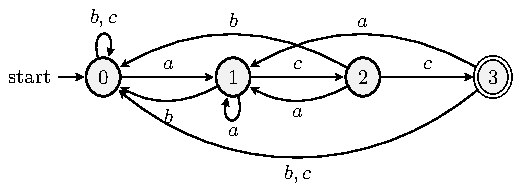
\includegraphics[width=0.35\textwidth]{./chapters/figures/forecasting/dfasr.pdf}
%\label{fig:dfa_adc}
%
%\hfill
%
%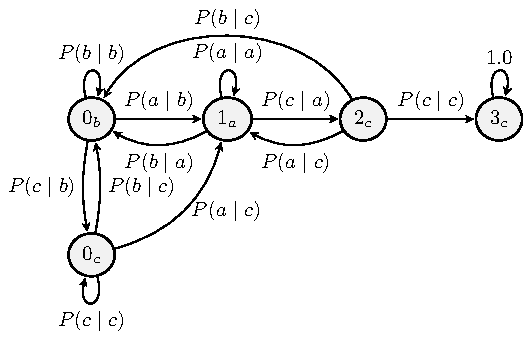
\includegraphics[width=0.35\textwidth]{./chapters/figures/forecasting/pmcr1.pdf}
%\label{fig:mc_adc}
%
%%\hfill
%\caption{DFA and PMC for $\mathcal{P}=a ; c ; c$,  $\Sigma=\{a,b,c\}$, and order $m=1$.}
%\label{fig:dfa_mc}
%\end{centering}
%\end{figure}

\begin{figure}[!h]
	\begin{centering}
		
	
			
			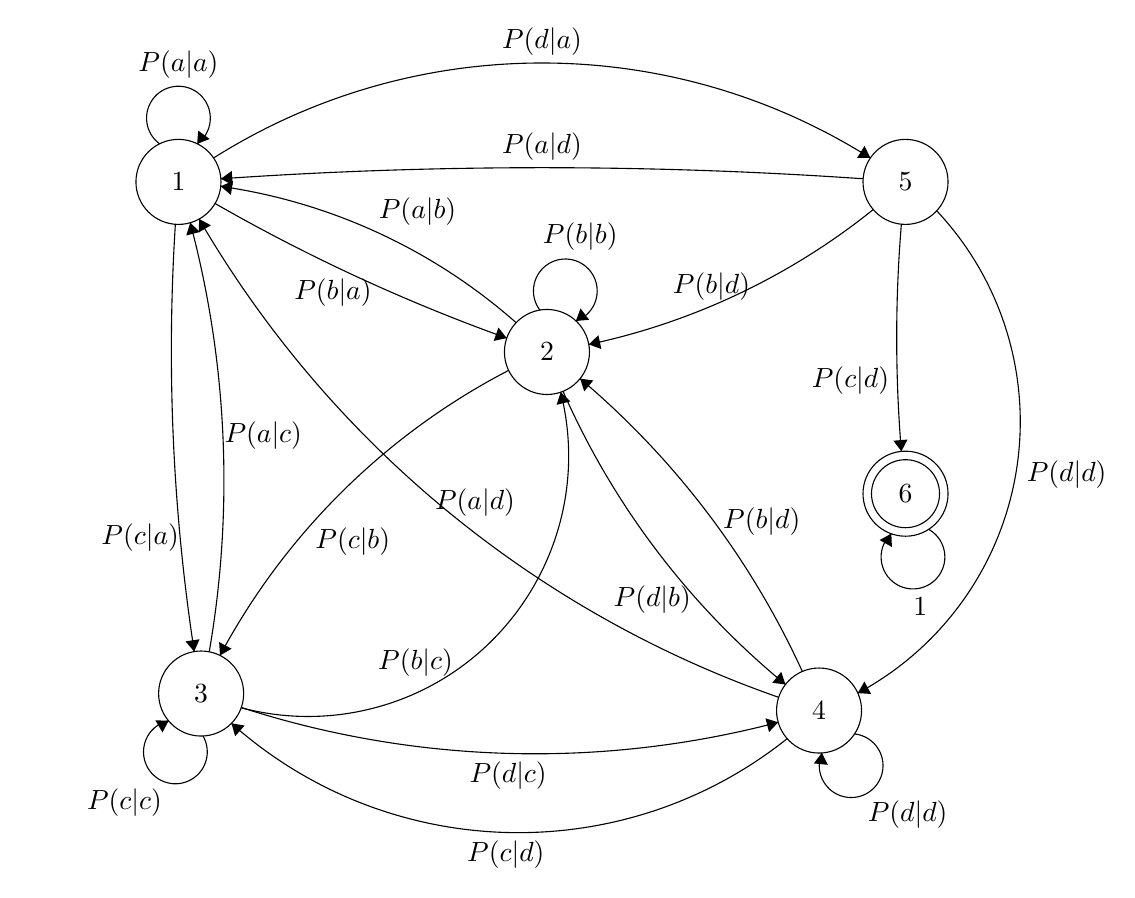
\begin{tikzpicture}[scale=.18]
			\tikzstyle{every node}+=[inner sep=0pt]
			\draw [black] (4.6,-12.2) circle (3);
			\draw (4.6,-12.2) node {$1$};
			\draw [black] (30.6,-24.2) circle (3);
			\draw (30.6,-24.2) node {$2$};
			\draw [black] (6.2,-48.3) circle (3);
			\draw (6.2,-48.3) node {$3$};
			\draw [black] (49.8,-49.5) circle (3);
			\draw (49.8,-49.5) node {$4$};
			\draw [black] (55.9,-12.2) circle (3);
			\draw (55.9,-12.2) node {$5$};
			\draw [black] (55.9,-34.2) circle (3);
			\draw (55.9,-34.2) node {$6$};
			\draw [black] (55.9,-34.2) circle (2.4);
			\draw [black] (3.277,-9.52) arc (234:-54:2.25);
			\draw (4.6,-4.95) node [above] {$P(a|a)$};
			\fill [black] (5.92,-9.52) -- (6.8,-9.17) -- (5.99,-8.58);
			\draw [black] (30.106,-21.253) arc (217.25487:-70.74513:2.25);
			\draw (32.95,-17.1) node [above] {$P(b|b)$};
			\fill [black] (32.64,-22.01) -- (33.58,-21.93) -- (32.97,-21.13);
			\draw [black] (6.328,-51.286) arc (30.18097:-257.81903:2.25);
			\draw (0.79,-55) node [below] {$P(c|c)$};
			\fill [black] (3.91,-50.22) -- (2.97,-50.19) -- (3.47,-51.05);
			\draw [black] (5.714,-45.34) arc (-171.29151:-183.63296:140.372);
			\fill [black] (5.71,-45.34) -- (6.09,-44.47) -- (5.1,-44.62);
			\draw (4.67,-37.32) node [left] {$\mbox{ }\mbox{ }\mbox{ }\mbox{ }\mbox{ }\mbox{ }\mbox{ }\mbox{ }P(c|a)$};
			\draw [black] (7.079,-10.512) arc (122.2697:57.7303:43.399);
			\fill [black] (53.42,-10.51) -- (53.01,-9.66) -- (52.48,-10.51);
			\draw (30.25,-3.31) node [above] {$P(d|a)$};
			\draw [black] (7.583,-12.513) arc (81.8726:48.57712:40.066);
			\fill [black] (7.58,-12.51) -- (8.3,-13.12) -- (8.45,-12.13);
			\draw (21.47,-15.28) node [above] {$P(a|b)$};
			\draw [black] (7.532,-45.612) arc (151.86818:117.42301:48.336);
			\fill [black] (7.53,-45.61) -- (8.35,-45.14) -- (7.47,-44.67);
			\draw (16.9,-36.53) node [below] {$P(c|b)$};
			\draw [black] (47.431,-47.66) arc (-129.36992:-156.24084:55.875);
			\fill [black] (47.43,-47.66) -- (47.13,-46.77) -- (46.5,-47.54);
			\draw (40.79,-41.65) node [left] {$P(d|b)$};
			\draw [black] (46.917,-50.329) arc (-75.2387:-107.9144:67.363);
			\fill [black] (46.92,-50.33) -- (46.02,-50.05) -- (46.27,-51.02);
			\draw (27.86,-53.1) node [below] {$P(d|c)$};
			\draw [black] (5.432,-15.082) arc (14.88666:-9.81113:70.847);
			\fill [black] (5.43,-15.08) -- (5.15,-15.98) -- (6.12,-15.73);
			\draw (7.81,-30.13) node [right] {$P(a|c)$};
			\draw [black] (27.764,-23.221) arc (-109.71785:-119.83243:128.561);
			\fill [black] (27.76,-23.22) -- (27.18,-22.48) -- (26.84,-23.42);
			\draw (15.5,-19.0) node [below] {$P(b|a)$};
			\draw [black] (31.568,-27.036) arc (14.17669:-104.88549:18.382);
			\fill [black] (31.57,-27.04) -- (31.28,-27.93) -- (32.25,-27.69);
			\draw (24,-46.09) node [left] {$P(b|c)$};
			\draw [black] (7.592,-11.979) arc (93.95767:86.04233:328.286);
			\fill [black] (7.59,-11.98) -- (8.42,-12.42) -- (8.36,-11.43);
			\draw (30.25,-10.7) node [above] {$P(a|d)$};
			\draw [black] (53.622,-14.151) arc (-51.2137:-78.03555:47.886);
			\fill [black] (33.55,-23.67) -- (34.44,-23.99) -- (34.23,-23.02);
			\draw (44.97,-20.61) node [above left] {$P(b|d)$};
			\draw [black] (55.607,-31.214) arc (-175.27936:-184.72064:97.384);
			\fill [black] (55.61,-31.21) -- (56.04,-30.38) -- (55.04,-30.46);
			\draw (54.78,-27.2) node [above left] {$P(c|d)$};
			\draw [black] (58.099,-14.237) arc (43.2333:-61.80904:21.727);
			\fill [black] (52.53,-48.27) -- (53.47,-48.33) -- (53,-47.45);
			\draw (64.42,-32.85) node [right] {$P(d|d)$};
			\draw [black] (52.291,-51.151) arc (84.18903:-203.81097:2.25);
			\draw (56.05,-55.84) node [below] {$P(d|d)$};
			\fill [black] (50,-52.48) -- (49.43,-53.23) -- (50.42,-53.33);
			\draw [black] (47.55,-51.483) arc (-51.43786:-131.71524:30.426);
			\fill [black] (8.34,-50.4) -- (8.6,-51.31) -- (9.27,-50.56);
			\draw (27.7,-58.68) node [below] {$P(c|d)$};
			\draw [black] (32.939,-26.078) arc (49.80232:24.58692:59.422);
			\fill [black] (32.94,-26.08) -- (33.23,-26.98) -- (33.87,-26.21);
			\draw (43,-36.14) node [right] {$P(b|d)$};
			\draw [black] (46.949,-48.567) arc (-109.23723:-149.82312:76.434);
			\fill [black] (6.06,-14.82) -- (6.03,-15.77) -- (6.89,-15.26);
			\draw (22.67,-34.85) node [right] {$P(a|d)$};
			\draw [black] (57.526,-36.707) arc (60.70628:-227.29372:2.25);
			\draw (56.94,-41.49) node [below] {$1$};
			\fill [black] (54.9,-37.02) -- (54.07,-37.47) -- (54.94,-37.96);
			\end{tikzpicture}
			
		
		
		%\hfill
		\caption{\pmconer for $\mathcal{P}=a ; d ; c$ with $\Sigma=\{a,b,c,d\}$, and order $m=1$.}
		\label{fig:pmc}
	\end{centering}
\end{figure}





%\end{comment}

\subsubsection*{Constructing the Pattern Prediction Model}
\label{sec:pmc_prediction}

~\citet{alevizos2017event} proposed to use the constructed \pmcmr to build a probabilistic prediction model that describes the DFA's run-time behavior. The method is based on calculating the \textit{waiting-time} distributions. Given a specific state of the \pmcmr, a \textit{waiting-time} distribution provides the probability of reaching an absorbing state in $n$ transitions from the current state. So by mapping the final states of the DFA to absorbing states of the \pmcmr by adding self-loops with probabilities equal to $1.0$. Therefore, we can calculate the probability of reaching a final state in $n$ transitions, which means predicting a full match of the defined pattern $\mathcal{P}$.

\par We denote by $W_{\mathcal{P}}(q)$ the waiting-time random variable that represents the number of transitions from a current state $q$ of DFA to reach a final state \cite{alevizos2017event}, where it also represents the expected number of future events from the current time event to a full match of the pattern $\mathcal{P}$, which is given by 

\begin{equation*}
W_{\mathcal{P}}(q)=inf\{n: q_{0},q_{1},...,q_{n}, q_{0}=q, q \in Q \backslash F, q_{n} \in F\}
\end{equation*}

where $Q$ is the set of states of the DFA, and $F$ the set of the  all final states. However, the \textit{waiting-time} distribution of the $W_{\mathcal{P}}(q)$ random variable can be computed based on the transition probability matrix $\Pi$ of the \pmcmr, where it has $h$ non-final states and $d$ final states (absorbing states) \cite{alevizos2017event}, then the distribution is calculated by the following equation 

\begin{equation*}
P(W_{\mathcal{P}}(q)=n)=\boldsymbol{\xi_{q}}\boldsymbol{N}^{n-1}(\boldsymbol{I}-\boldsymbol{N})\boldsymbol{1}
\end{equation*}
where $\boldsymbol{N}$ is $h \times h$ matrix that obtained by re-arranging the transition matrix $\Pi$ to include transitions between the non-final states of the DFA, $\boldsymbol{I}$ is an identity matrix of size $h \times h$, and  $\boldsymbol{1}$ is a $h$-dimensional vector of ones. The $\boldsymbol{\xi_{q}}$ is $1 \times h$ row of elements that contains zeros except $1.0$ in the cell corresponding to $q$. 
\par Finally, the model provides the prediction reports in the form of intervals i.e.,  $I=(\mathit{start},\mathit{end})$. Which means that the DFA is expected to reach a final state  after future transitions (number of events $n$) between $\mathit{start}$ and $\mathit{end}$ with probability $P(I)$ at least some constant threshold $\theta_{p}$ that defined by the user, given by:
\begin{equation*}
P(I)=\sum_{n \in I}{P(W_{\mathcal{P}}(q)=n)}\ where\  P(I) \geq \theta_{p} 
\end{equation*}
where $P(I)$ equals the sum of probabilities of all number of future events $n$ that fall within $I$ ($start\leq n\leq end$). Furthermore, the length of the intervals ($spread(I) = end - start$)  can be restricted to not be greater than a maximum spread threshold $\theta_{s}$ ($spread(I)\leq \theta_{s}$)



\begin{figure}[H]
	\begin{centering}
		\center
		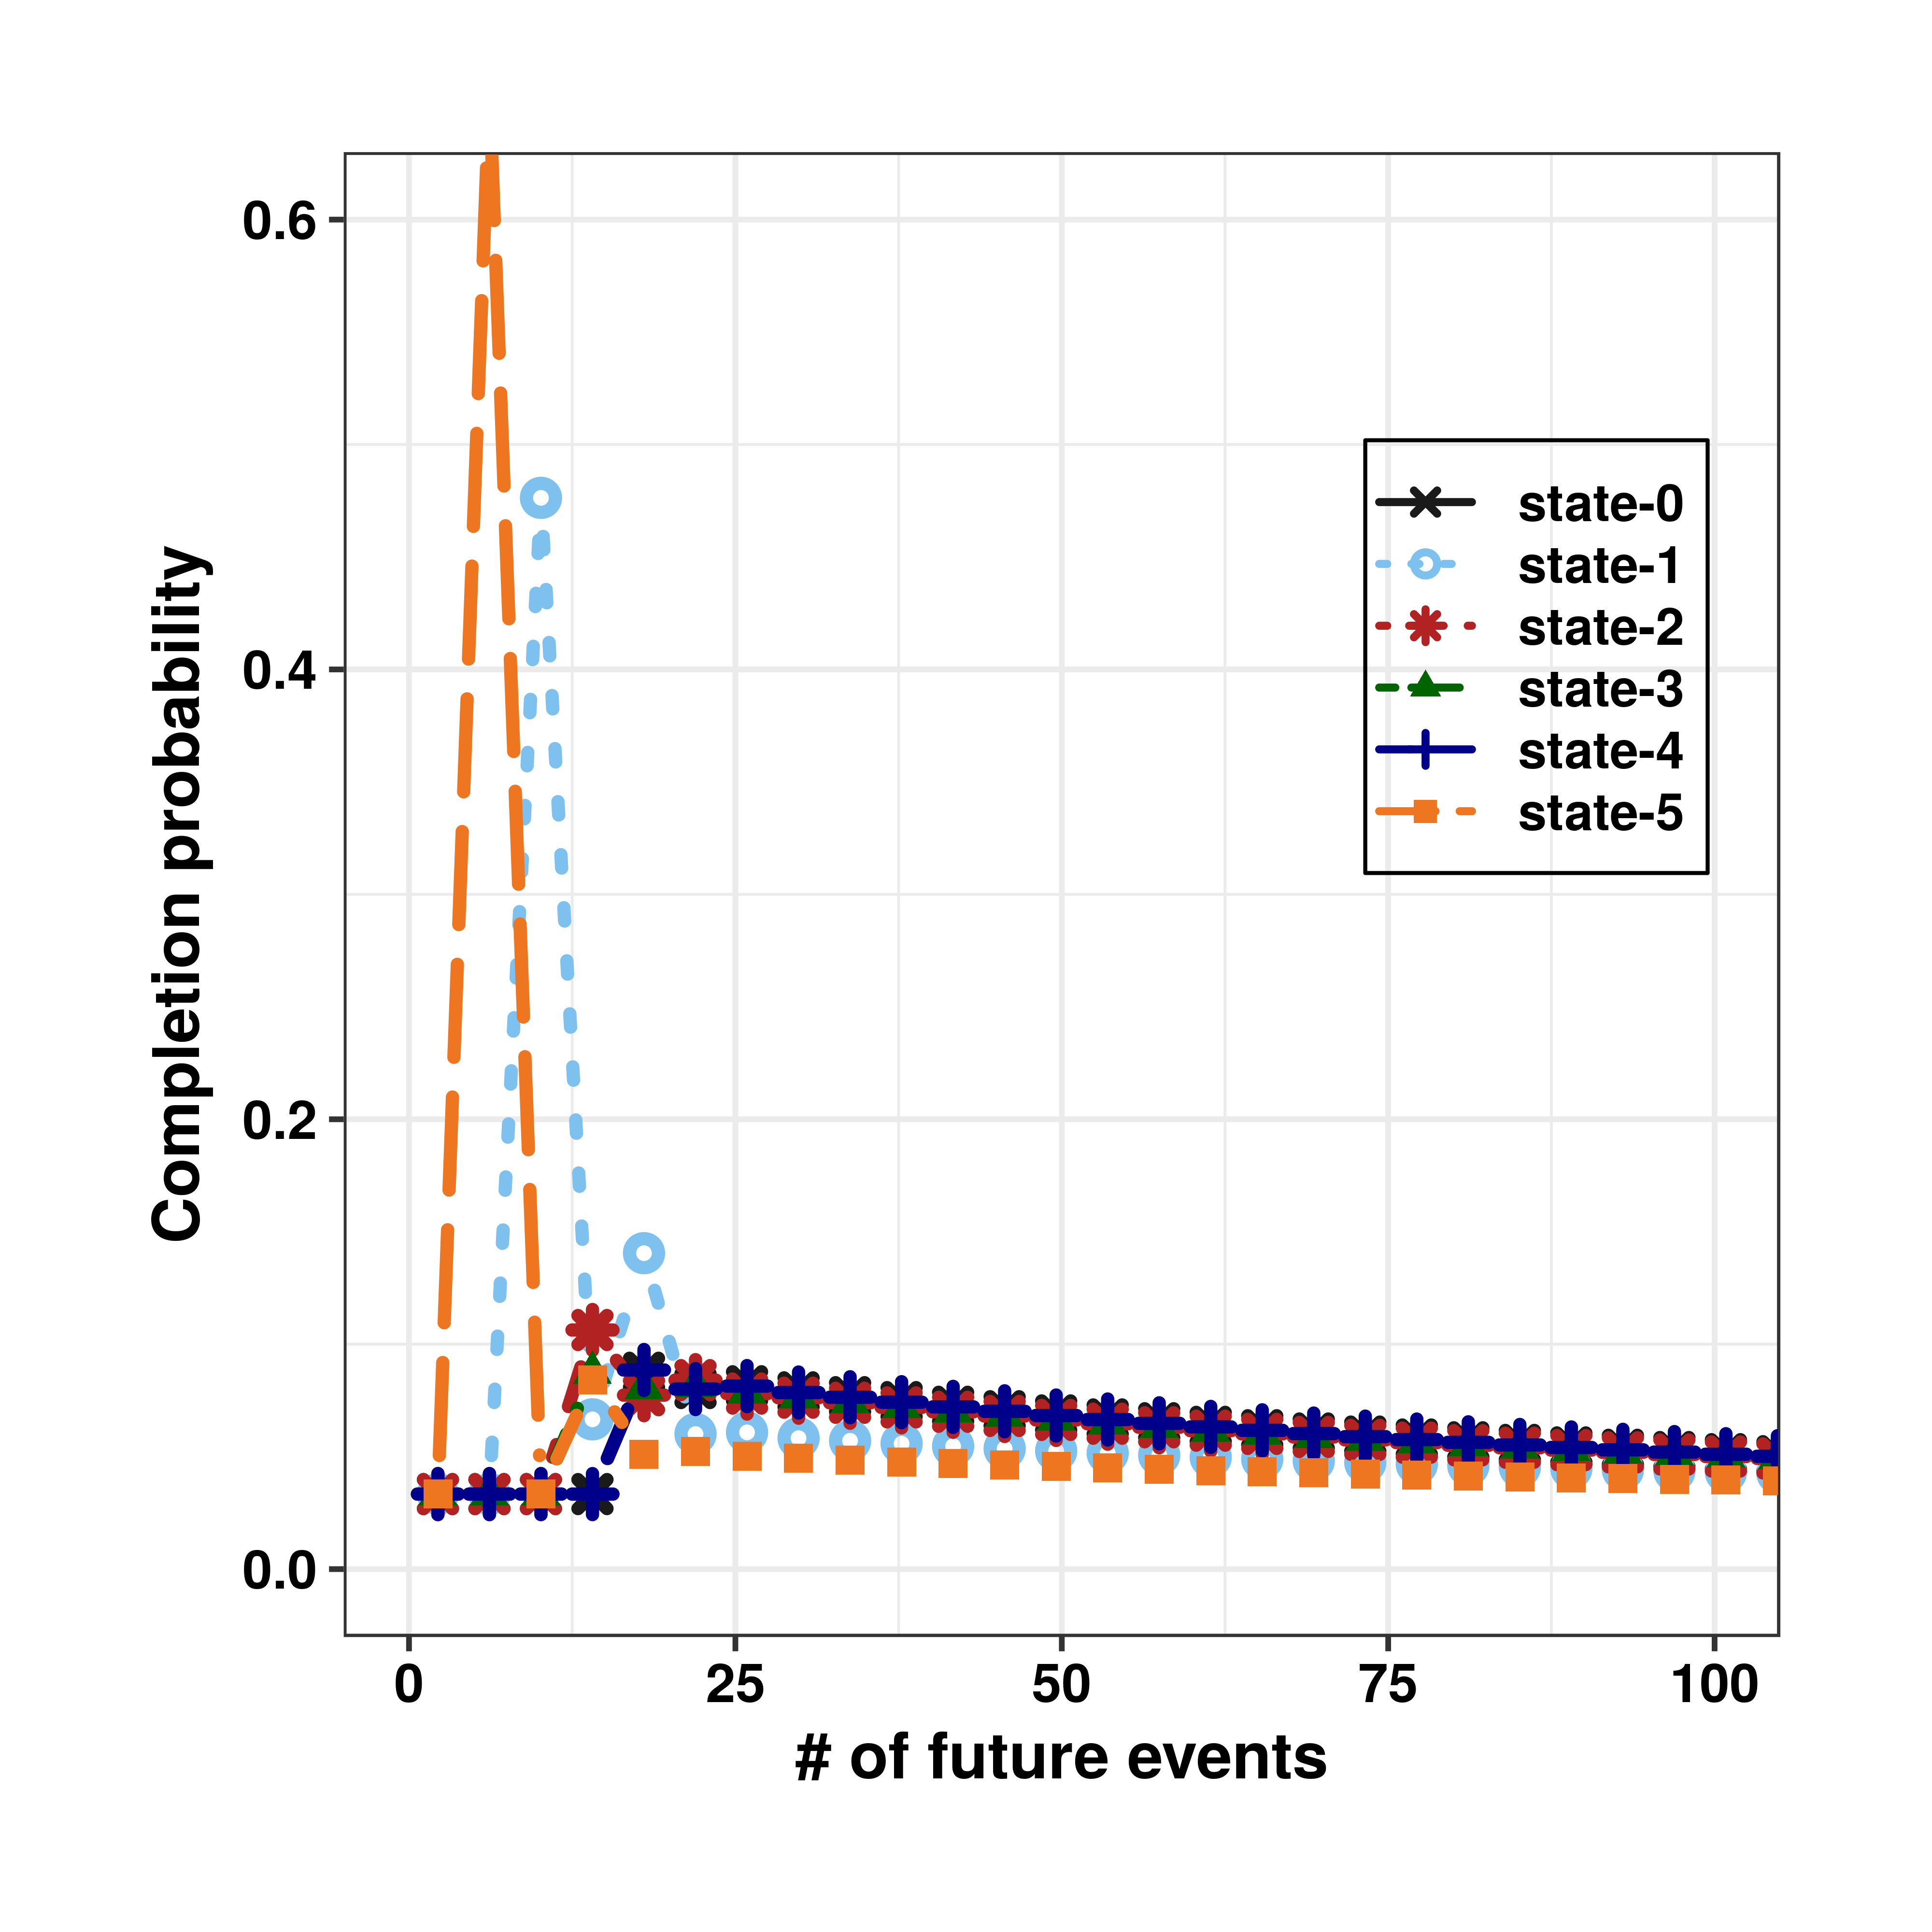
\includegraphics[width=\textwidth,keepaspectratio]{chapters/figures/new_wt.png}
		
		
		\caption{Waiting-time distribution for
			$\mathcal{P}=a ; d ; c$, $\Sigma=\{a,b,c,d\}$, $m=1$, $\theta_{p}=0.5\ and\ \theta_{s}=20$.}
		\label{fig:wt1}
	\end{centering}
\end{figure}

\par These intervals are estimated by a single-pass algorithm that scans a waiting-time distribution and finds the smallest (in terms of length) interval that exceeds the $\theta_{p}$ and has a spread  not greater that $\theta_{s}$. For example, Figure~\ref{fig:wt1} shows the \textit{waiting-time} distributions for all non-final states of the DFA presented in Figure~\ref{fig:wt1}, and the generated intervals are depicted in Figure~\ref{fig:predictionsIntervals}.


\begin{figure}[H]
	\begin{centering}
		\center
			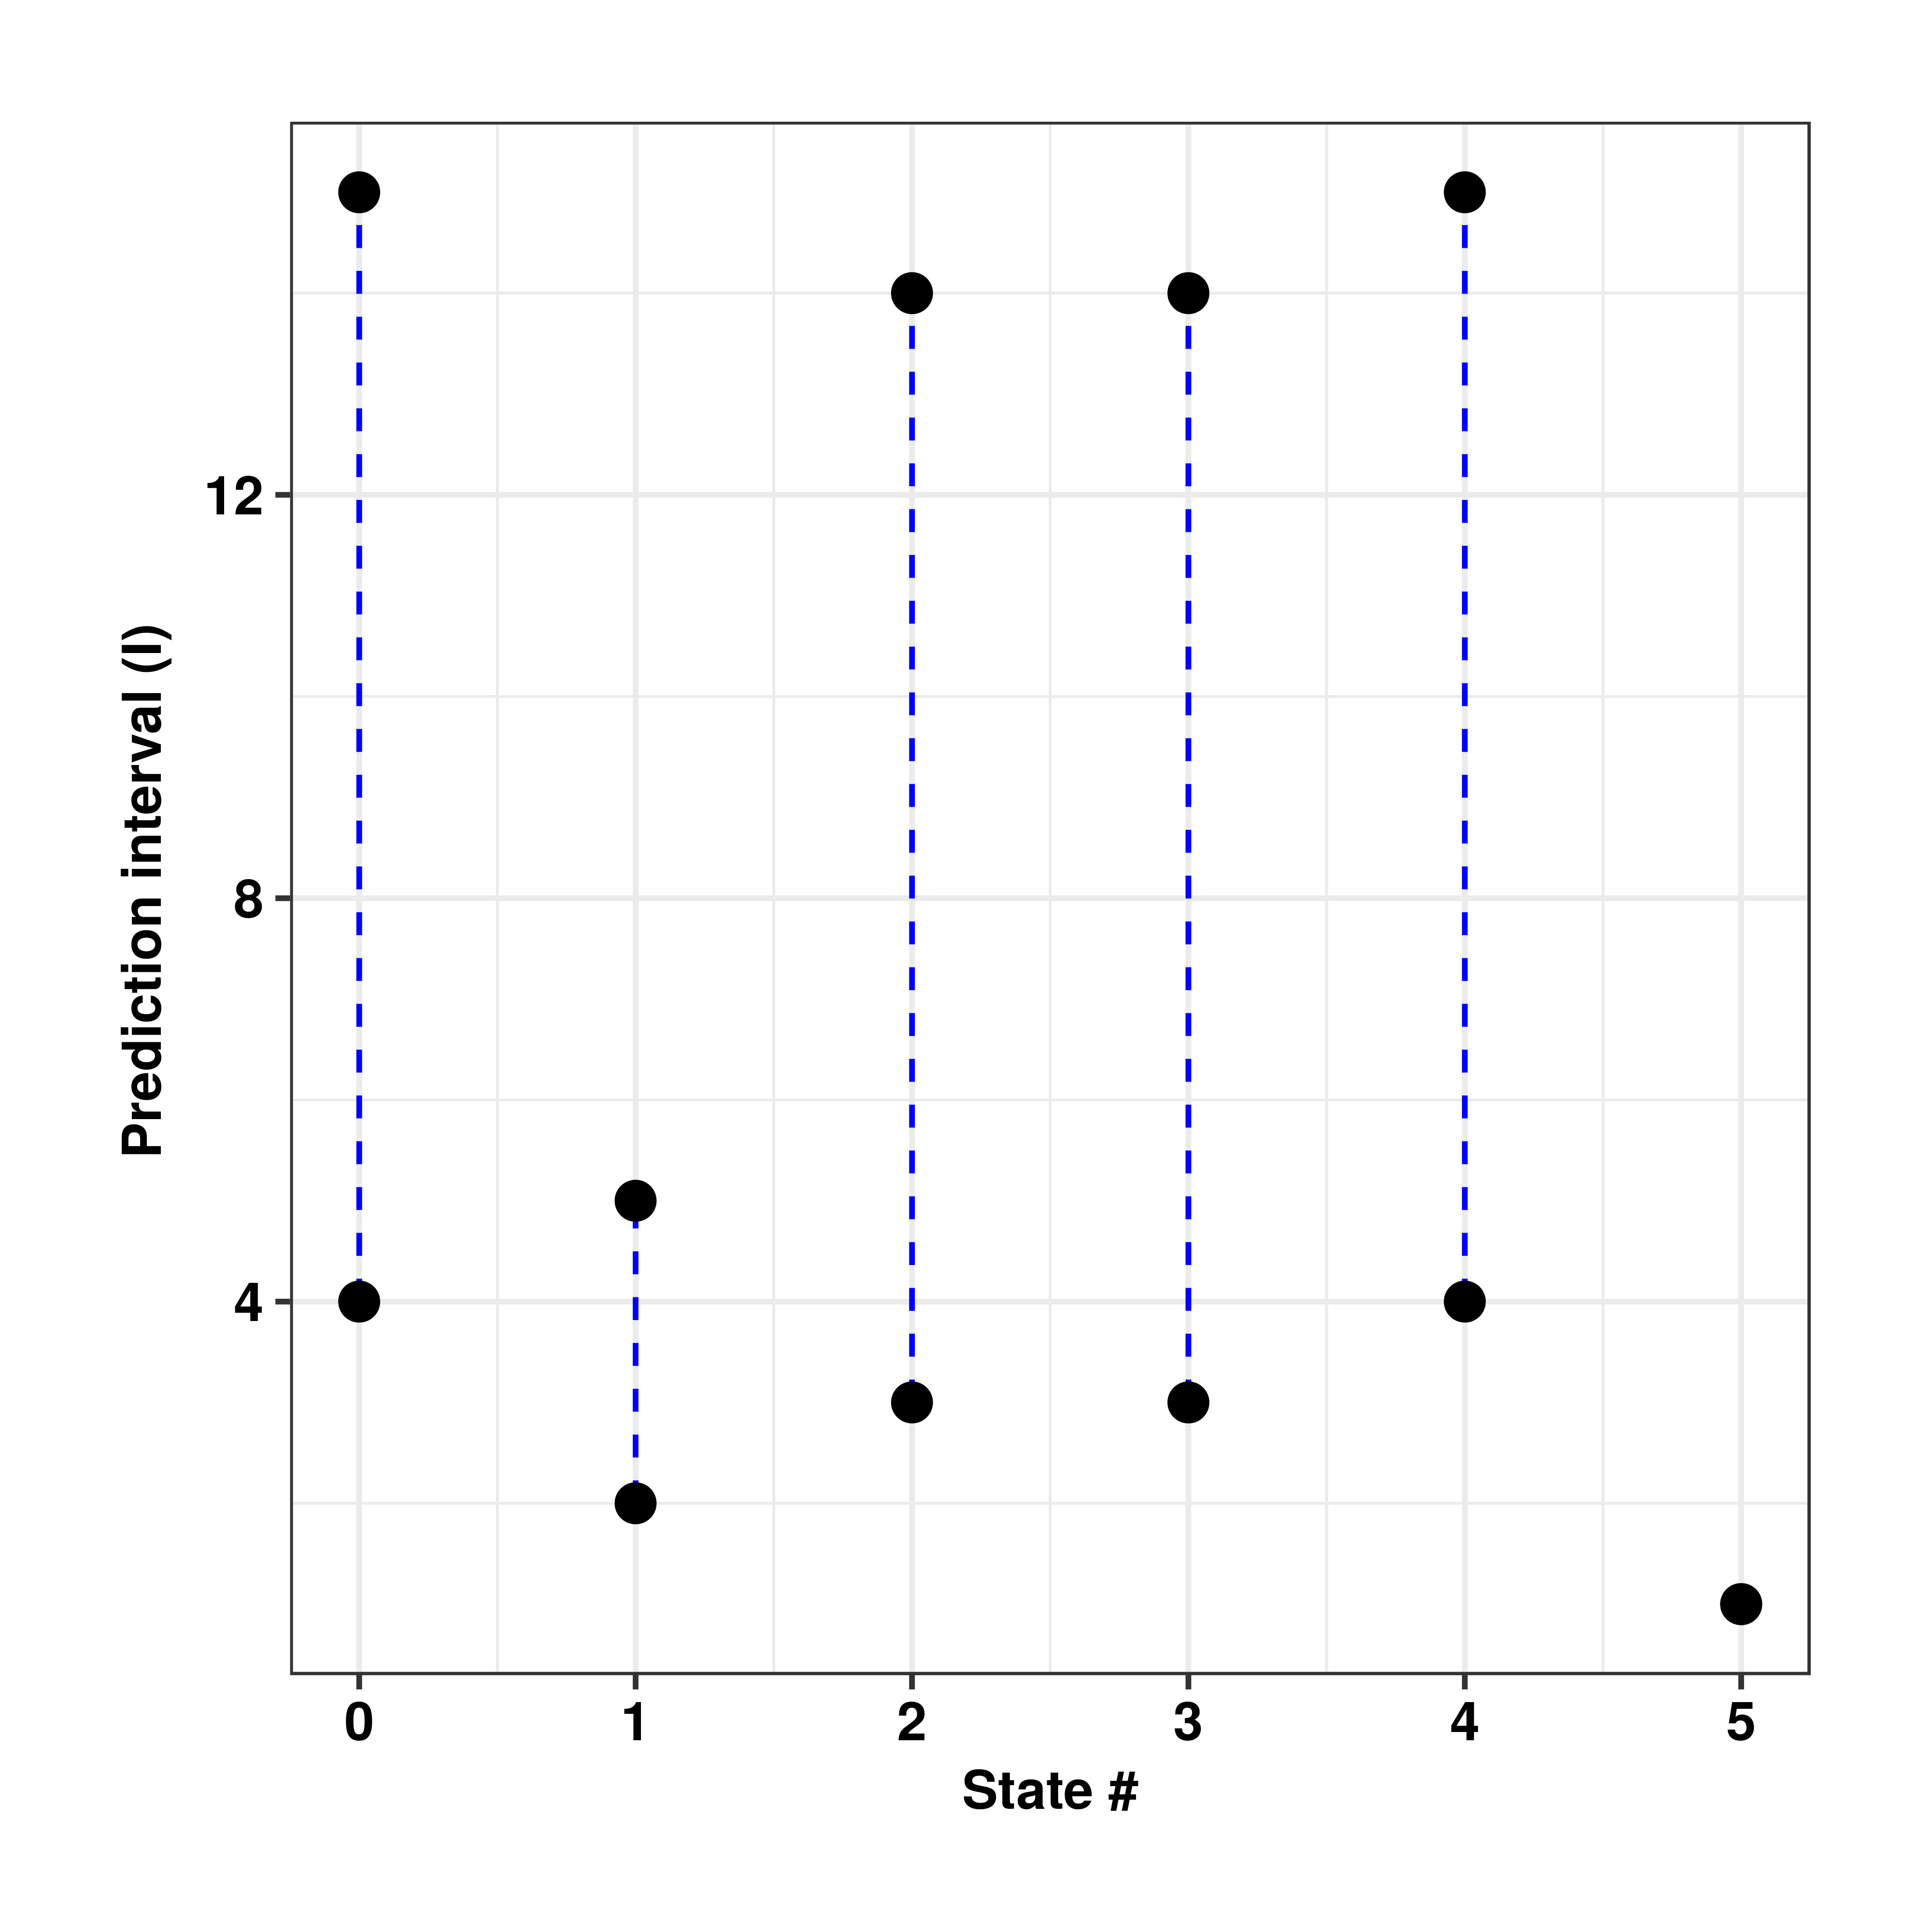
\includegraphics[width=\textwidth,keepaspectratio]{chapters/figures/new_prediction_intervals.png}
					
		\caption{Example of the computed prediction intervals for
			$\mathcal{P}=a ; d ; c$, $\Sigma=\{a,b,c,d\}$, $m=1$, $\theta_{p}=0.5\ and\ \theta_{s}=20$.}
		\label{fig:predictionsIntervals}
	\end{centering}
\end{figure}

\par The proposed method assumes that the transition probability matrix $\Pi$ is available to build the prediction intervals. However, this is not true in the real-world applications.
Therefore, it is essential to learn the values of the \pmcmr's transition probability matrix in order apply this method. One common way, is to use the maximum-likelihood estimator to learn the transition probabilities as illustrated in Section ~\ref{sec:theoretical}. 

\par This model is performing the learning over an event stream $s$, which is usually has a slow convergence to a sufficiently good model. Where in the case of multiple event streams, a unique model associated with each stream is needed. Accordingly, we present in this work, a technique to share information among the \pmcmr predictors over multiple input event streams (i.e., distributed learning of the transition probability matrix).

\section{Pattern Prediction over Multiple Event Streams}

We extend the pattern prediction problem over a single event stream to the case of multiple distributed input event streams, where there is an associated prediction model for each event stream. We further present our proposed cooperative learning based approach by using a distributed online prediction protocol \cite{kamp2014communication} to synchronize the distributed prediction models in a communication-efficient manner. 


\subsection{Extended Problem Formulation}

\par In this section, we extend the problem of pattern prediction over a single event stream to consider the setting where there are multiple input event streams. Let $O = \{ o_1, ..., o_k\}$ be a set of \emph{$K$} objects/entities (e.g., moving objects), each of which is generating an event stream $s_i$, hence, we have a set of real-time input event streams $S = \{ s_1, ..., s_k\}$, where these streams are produced independently from the same distribution.


 \par $\mathcal{P}$ is a user-defined pattern given in the form of regular expression, which is monitored in every stream $s_i \in S$. Then, we have a system consists of \emph{$K$} local predictor (learner) nodes $n_1,n_2\dots,n_k$, each of which receives an input event stream $s_i\in S$ that is associated with a single object $o_i \in O$.

\par  The goal is to provide online predictions about the completion of the pattern $\mathcal{P}$ within each stream $s_i$. Each node maintains a local prediction model $f_i$. Then for each new arriving event tuple  $e_t \in s_i$, the $f_i$ model provides an online prediction interval about the future full match of the pattern $\mathcal{P}$.

\par In other words, we have separated running instances of an online prediction algorithm on distributed nodes for \emph{$K$} input event streams. For example, massive streams of events that describe trajectories of group of moving vessels in the context of maritime monitoring, where there is one predictor node for each vessel's event stream.
  
  
  \par In this work, we employ the \pmcmr models on the distributed predictor nodes, each model is associated with a particular event stream. While these predictors can work in isolation with no communication with other local predictors, such non-cooperative way leads to inefficiency in terms of learning convergence and predictive performance among all predictors. Thus, in this work, we propose to use the distributed online prediction protocol \cite{kamp2014communication} to enable the communication among the local predictors to synchronize their models.     
%
%The defined pattern $\mathcal{P}$ is monitored over each event stream $s_i$  by a  predictor nodes  $n_i$  that maintains a local prediction model $f_i$, where there is one node for each vessel's event stream.  The prediction model $f_i$ gives the ability to provide an online predictions about when the pattern will be completed in the form of an expected number of future events before a full match does occur.

\subsection{The Proposed Method}
\label{sec:proposed_approach}

\par This work proposes a scalable and distributed prediction system for user-defined patterns over multiple massive input event streams. The system  uses the PMC forecasting method \cite{alevizos2017event} as the base prediction model, where there is a \pmcmr model associated with each input event stream $s_i$ on a predictor node $n_i$. And it employs the distributed online learning protocol \cite{kamp2014communication} to exchange information among the distributed predictors of the input event streams, which allows to synchronize the parameters of their prediction models, which are represented by the transition matrices.

%
%Thus, the prediction model $f_i$ on a predictor node is represented by \pmcmr and its associated DFA.

\subsection*{Distributed Online Learning for Pattern Prediction}

\par In what follows, we describe the details of adapting the distributed online learning protocol \cite{kamp2014communication} with the pattern prediction (\pmcmr) models. This protocol provides a communication-efficient dynamic synchronization scheme based on a periodic static scheme.


\par Algorithm~\ref{algonline:dol} presents the distributed online prediction protocol by dynamic model synchronization on both the predictor nodes and the coordinator. We refer to the PMC's transition matrix $\boldsymbol{\Pi}_i$ on predictor node $n_i$ by $w_i$, which represents the parameters of the local prediction model $f_i$. 

\par That is, when a predictor $n_i:\ i \in[k]$ observes an event $e_j$ it revises its internal model state ($w_i$) and provides a prediction report. Then it checks the local conditions, by checking the local model divergence from a reference model $w_r$ after consuming a predefined number of events (batch size $b$), to decide whether there is a need to synchronize its local model with the coordinator [or not]. $w_r$ is maintained in the predictor node as a copy of the last computed aggregated model $\hat{w}$ from the previous full synchronization step, which is shared among all distributed predictors.
%define delta%
 \par Let $\Delta$ be a predefined divergence threshold parameter. Then, by monitoring the local condition $(\|w_i - w_r\|^2 > \Delta)$ on all local predictors, we have a guarantee that if none of the local conditions is violated, the divergence (i.e., variance of local models $\delta(w)=\frac{1}{k} \sum_{j=1}^{k}\|w_i - \hat{w}\|^2$) does not exceed the threshold $\Delta$ \cite{kamp2014communication}. This is the key point of this protocol that reduces the communication overhead in comparison to the static based communication scheme, where the predictors always communicate periodically after observing a fixed number ($b$) of events ~\cite{dekel2012optimal}.  

\par On the other hand, the coordinator receives the parameters of prediction models from the predictor nodes that requested for model synchronization (violation). Then it tries to keep incrementally querying other nodes for their local prediction models until reaching out all nodes have been queried, or the variance of the aggregated parameters $\hat{w}$ that is computed from the already received models is less or equal than the divergence threshold $\Delta$. The coordinator uses a synchronization operation to compute the parameters of a global model  $\hat{w}$. Finally, $\hat{w}$ is sent back to the predictor nodes that sent their models after the violation or have been queried by the coordinator. 

\begin{algorithm}[h]
	\caption{Communication-efficient Distributed Online Learning \cite{kamp2014communication}.} 
	\begin{algorithmic}[1] 
		
		\Statex \Indm  \textbf{Predictors:}
		\Statex \Indp node $n_i$: at observing event $e_j$
		
		\Statex \Indp update the parameters of the local prediction model $w_i$ and provide a prediction interval $I$ \;
	 

		\Statex \If {$j\mod b = 0\ and\ \|w_i - w_r\|^2 > \Delta$}  
		\Statex send  $w_i$ to the Coordinator (violation) \;
		\Statex \Indm \textbf{Coordinator}:
		\Statex \Indp receive parameters of local models with violation 
		 $B=\{w_i\}_{i=1}^m$ \;
	
	
		\Statex \While{$|B| \neq k $ and $\frac{1}{|B|} \ \sum_{w_i\in  \Pi}\|w_i - \hat{w}\|^2 > \Delta$}{
			
			 \Statex  \hspace{\algorithmicindent} add other nodes that have not reported violation for \Statex \hspace{\algorithmicindent} their models $ B \gets \{w_l : w_l \notin B\ and\ l \in [k]\}$    \;
			\Statex  \hspace{\algorithmicindent} receive models from nodes in $B$\;
	}
        \Statex
		\Statex compute a new global model $\hat{w}$ \;
		\Statex send $\hat{w}$ to all the predictors in $B$ and set $w_{1}\dots w_{m}=\hat{w} $\; 
		\Statex \If {$|B| = k$}{
		\Statex  \hspace{\algorithmicindent} set a new reference model $w_r	\gets \hat{w}$ \; }
	
	\end{algorithmic}
	\label{algonline:dol}
\end{algorithm}


\par  We use this protocol for the pattern prediction models, which are internally based on the \pmcmr. This allows the distributed \pmcmr predictors for multiple event streams to synchronize their models (i.e., the transition probability matrix of each predictor), and learn a shared model in a communication-efficient way. 


\subsection*{Learning a Global Transition Probability Matrix}

\par We propose a \textit{synchronization operation} for the transition probability matrices ($w_i=\boldsymbol{\Pi}_i :i \in[k]$) of the $k$ distributed \pmcmr predictors. The operation is based on distributing the maximum-likelihood estimation \cite{anderson1957statistical} for the transition probabilities of the \pmcmr models. 
Let $\pi_{i,j}$ the transition probability from state $i$ to state $j$ 
and $n_{k,i,j}$ the number of transitions from state $i$ to state $j$ on node $k$. Then, the global estimation $\hat{\pi}_{i,j}$ for $p_{i,j}$ is described by:

\begin{equation}
\label{eq:dis_pi_estim}
\hat{\pi}_{i,j} = \frac{\sum_{k \in K} n_{k,i,j}}{\sum_{k \in K} \sum_{l \in L} n_{k,i,l}}
\end{equation}

That is,  $\hat{\Pi}$ is the global transition probability matrix that will be shared among all \pmcmr predictors. 
\par Moreover, we measure the divergence of the local models from the reference model $\|w_i - w_r\|^2$ by calculating the sum of square difference between the local transition probability matrix $\Pi_i$ and the reference transition matrix $\Pi_r$:
\begin{equation*}
\label{eq:dis_pi_varinace}
\|w_i - w_r\|^2=|\Pi_i - \Pi_r\|^2=\sum_{l,j} (\pi{i,l,j} -\pi{r,l,j})^2
\end{equation*}

Where $\pi{i,l,j}$ is the transition probability from state $l$ to state $j$ in the $\Pi_i$, and the $\pi{r,l,j}$ the reference transition probability.
\section{Analysis of the Proposed Approach}

\subsection{General  Overview}
\par Generally, our approach relies on enabling the collaborative learning among the distributed predictors. Each predictor node receives a stream of events related to a distinct moving object, and the central coordinator is responsible of synchronizing their prediction models using the \textit{synchronization operation}. Moreover, the predictors they only need to share the parameters of their models without aggregating all input event streams. 

\par In addition, our approach relies on enabling the collaborative learning between the prediction models of the input event streams. By doing so, we assume that the underlying event streams belong to the same  distribution and share the same behavior (e.g., mobility patterns). We claim this assumption is reasonable in many application domains: for example, in the context of maritime surveillance, vessels travel through standard routes, defined by the International Maritime Organization (IMO). Additionally, vessels have similar mobility patterns in specific areas such as moving with low speed and multiple turns near the ports \cite{pallotta2013vessel,liu2014knowledge}. That allows our system to construct a coherent global prediction model dynamically for all input event streams based on merging their local prediction models.

\par The underlaying learning process is based on estimating the transition probability matrix of the \pmcmr models, where the maximum-likelihood estimator  \cite{anderson1957statistical} is used to learn the transition probability matrix for each \pmcmr. In our approach, we propose a synchronization operation (Equation ~\ref{eq:dis_pi_estim}) to build a global estimation of the transition probability matrix among the \emph{$K$} predictors. In next, we present the maximum-likelihood estimator, and we  provide a theoretical analysis of the proposed operation, where we further present a probabilistic guarantee of the efficiency of our distributed learning estimation against the isolated estimations.   
% may add it to conclusion 
%\par By enabling collaborative learning our approach is imposing an acceleration of learning of the underlying prediction models with less training data, in addition, it provides an improvement of the predictive performance compared to the no-distributed  version of event forecasting with Pattern Markov Chains system. 


\subsection{Theoretical Analysis}
\label{sec:theoretical}

 In this section, we present preliminaries of the Markov chain models and the maximum-likelihood estimator of the transition probabilities, and we describe the theoretical properties of our proposed synchronization operator and its relation with the maximum-likelihood estimator. Also, we derive a probabilistic guarantee of our method estimations for the transition probabilities. 
 
 
 \subsubsection*{Preliminaries}
 We first give a brief introduction to the Markov chain theory, where the theoretical definitions and notations presented are based on the work described in \cite{bertsekas2002introduction,Billingsley1961,anderson1957statistical,howard2012dynamic}.

\begin{definition}
	Let $\{q_0, q_1, \ldots q_n\}$ be a sequence of random variables as \textbf{Markov chain}, where the variable $q_i$ belongs to a finite state space $\mathbf{S =\{1,\ldots m\}}$ and represents the observed state of the chain at time $i$. Let the transition probabilities of the Markov chain $p_{ij}(t+1)$ such that $i,j \in S$ and $t=0,\ldots, n$, where  $p_{ij}(t+1)$ is the probability of the state $j$ at time $t+1$, given  state $i$ at time $t$, then the sequence $\{q_0, q_1, \ldots q_n\}$ satisfies the \textbf{Markov property} 
	
	\begin{equation}
	\begin{aligned}
	P(q_{t+1}=j|q_{t}=i,q_{t-1}=i_{t-1},\ldots ,q_{0}=i_{0})=P(q_{t+1}=j|q_{t}=i)\\
	\forall i,j,i_{t-1},i_{0} \in S
	\end{aligned}
	\end{equation}

\end{definition}



\par That is, the probability of moving to a future state only depends on the current state (Markov chain of order $1$). While for higher order $m$ Markov chains the conditional probabilities are modeled to be dependent on the last $m$ states. 

\par When the conditional probabilities $P(q_{t+1}=j|q_{t}=i)$ are independent of the time $t$, the Markov chain is called \textbf{homogeneous} such that $p_{ij}:=P(q_{t+1}=j|q_{t}=i)$.

The transition probabilities of the Markov chain are represented by a $m \times m$ matrix that called \textbf{transition probability matrix} $\boldsymbol{\Pi}$ with $p_{ij}$ elements


\begin{equation}
\label{eq:matrix_example}
\boldsymbol{\Pi} = 
\begin{bmatrix} 
p_{1,1}	   &p_{1,2}  &. 		&. 		& . &  	p_{1,m} \\
p_{2,1}		   &.  & .		& .	    & .	& . \\
. 		   &.  & .		& .	    & .	& . \\
.		   &.  & .		& .		& .	& . \\
.		   &.  & .		& .		& .	& .\\
p_{m,1}	   & p_{m,1}	&.		& .	& .	&p_{m,m}
\end{bmatrix}
\end{equation}

where $0 \leq p_{i,j}\leq 1 $ and the rows sum up to one 
\begin{equation}
\sum_{j=1}^{m} p_{i,j}= 1\ \ \ \ \ \ \ \ \ i=1,2 \ldots m
\end{equation}

\subsection{Learning the Transition Probability Matrix for a Single Markov Chain}
 \
\par As mentioned in Section ~\ref{sec:pmc_prediction}, we rely on the transition probability matrix of \pmcmr to build the prediction intervals. Given that the sequence of the states $\{q_0, q_1, \ldots q_n\}$ that DFA visits after consuming the input event stream is a 1-order Markov chain.


\par However, in practice the underlying transition probability matrix is unknown, and desirable to estimate or learn it form the observed sequence $\{q_0, q_1, \ldots q_n\}$. The maximum-likelihood estimator is a common method to estimate the transition probability matrix \cite{anderson1957statistical}.


\begin{definition}
	Let $\boldsymbol{\Pi}$ is the transition probability matrix of a single Markov chain with a set of states $S$, 
	$\pi_{i,j}$ the transition probability from state $i$ to state $j$,
	$n_{i,j}$ the number of observed transitions from state $i$ to state $j$,
	then the maximum-likelihood finds $\boldsymbol{\hat{\Pi}}$ as an estimate for $\boldsymbol{\Pi}$, where its elements $\hat{p}_{i,j}$ are
	\begin{equation}
	\label{eq:pi_estim}
	\hat{p}_{i,j}=\frac{n_{i,j}}{\sum_{l \in S} n_{i,l}}=\frac{n_{i,j}}{n_{i}}
	\end{equation}
	
\end{definition} 

Where this estimator is used separately to learn each transition probability matrix of all \pmcmr models.   


\textbf{Proprieties of the maximum-likelihood estimates}. 
	The maximum likelihood estimates of transition probabilities of a single sequence $\{q_0, q_1, \ldots q_n\}$  are obtained based on the observed transitions between the states of the chain. That is, the maximum likelihood estimates are basically the count of transitions from $i$ to $j$ divided by the total count of the chain being in state $i$.  
	
	\par ~\citet{anderson1957statistical} have shown that 
	
	
%	\begin{equation}
%	\label{eq:lim_dist}
%	\lim_{n\to\infty} \sqrt{n}\ (\hat{p}_{i,j} - {p}_{i,j}) \sim \mathcal{N}(\mu,\,\sigma^{2}_{mle})\,.
%	\end{equation}

	\begin{equation}
	\begin{aligned}
	\label{eq:lim_dist}
	 \sqrt{n}\ (\hat{p}_{i,j} - {p}_{i,j}) \xrightarrow{d} \mathcal{N}(\mu,\,\sigma^{2})\\
	 as\ n \xrightarrow{} \infty
	 \end{aligned}
	\end{equation}
Thus, the random variable $\sqrt{n}\ (\hat{p}_{i,j} - {p}_{i,j})$ has asymptotically normal distribution with mean $\mu=0$, and  variance  $\sigma^{2}$ is given by   

\begin{equation}
\begin{aligned}
\sigma^{2}=\mathrm{Var}(\sqrt{n}\ (\hat{p}_{i,j} - {p}_{i,j})) = \frac {{p}_{i,j}\ (1- {p}_{i,j})} {\phi_{i}} \\
\text{s.t.}\ \phi_{i} = \sum_{l=1}^{m} \sum_{t=1}^{n} \eta_{l} \ p_{l,j}^{t-1}
\end{aligned}
\end{equation}

Where $p_{l,j}^{t-1}$ is the probability of state $j$ at time $t-1$ given that the state $l$ at time $0$ ~\cite{anderson1957statistical}. We are interested in the variances of $(\hat{p}_{i,j} - {p}_{i,j})$ that represents the error in the estimation of ${p}_{i,j}$ by the maximum-likelihood estimator, which is given by:

	\begin{equation}
\begin{aligned}
\label{eq:var_isol}
	\mathrm{Var} (\hat{p}_{i,j} - {p}_{i,j}) =  \frac {\mathrm{Var}(\sqrt{n}\ (\hat{p}_{i,j} - {p}_{i,j}))}{n} = \frac {\sigma^{2}}{n} 
\end{aligned}
\end{equation}

It is clearly seen that variances are dropping as the sample size $n$ grows large.  In next, we will show that our proposed approach of synchronizing the maximum likelihood estimators over $k$ chains is preserving  a similar asymptotic behavior and gives efficient estimates of the transition probabilities.


\subsubsection{Probabilistic Learning Guarantee}
 %in Equation ~\ref{eq:dis_pi_estim}% 
\par The proposed synchronization operator is aggregating the maximum-likelihood estimates over $k$ observed sequences (i.e., sequences of the DFA states based on the consumed event streams), the operator estimates a global transition probabilities matrix for a set of $k$ sequences, which are arranged in serial order as one large chain with length $N=k*n$, where we assume that all $k$ sequences have $n$ observations. For the sake of simplicity, we assume that the synchronization phase happens on batch size equals $n$ (i.e., $b=n$) given that the $\Delta$ is zero, then the global transition probabilities $\hat{\pi}_{i,j}$ are given 
\begin{equation}
\label{eq:dis_pi_estim2}
	\begin{aligned}
\hat{\pi}_{i,j}=\frac{\sum_{k \in K} n_{k,i,j}}{\sum_{k \in K} \sum_{l \in L} n_{k,i,l}} = \hat{p}_{i,j}(N)\\\\
 where\ N = k*n.
 \end{aligned}
\end{equation}
%This is equivalent to

\par Thus, this operation it allows to observe more samples, which is naturally producing a better estimates of the transition probabilities. In addition, our proposed synchronization operation of the $k$ transition matrices has the same proprieties as the maximum likelihood estimator over a serial sequence of all $k$ sequences, but with skipping $k-1$ transitions between each two consecutive sequences, which is in practice a small number that can be neglected comparing to the total transitions count $k*n$. As result, the global transition probabilities of our approach  have the same properties as maximum likelihood estimates, in particular, the the random variable $\sqrt{N}\ (\hat{\pi}_{i,j} - {p}_{i,j})$ has asymptotically normal distribution with mean $\mu=0$, and  following Equation ~\ref{eq:lim_dist} we have variance 

\begin{equation}
\begin{aligned}
\label{eq:lim_dist2}
\sqrt{N}\ (\hat{\pi}_{i,j} - {p}_{i,j}) \xrightarrow{d} \mathcal{N}(0,\,\sigma^{2})\\
as\ N \xrightarrow{} \infty\\
where\ N = n*k .\\
\end{aligned}
\end{equation}

So, 
\begin{equation}
\begin{aligned}
\label{eq:var_sync}
 \mathrm{Var} (\hat{\pi}_{i,j} - {p}_{i,j}) = \frac {\sigma^{2}}{N} =  \frac {\sigma^{2}}{k*n}
\end{aligned}
\end{equation}


That is, since $N > n$ combining $k$ sequences, the variances of estimations of our method  $\mathrm{Var} (\hat{\pi}_{i,j} - {p}_{i,j})$ are smaller than the estimates of maximum-likelihood over a single sequence $\mathrm{Var} (\hat{p}_{i,j} - {p}_{i,j})$. 
\par Thus, it follows from the  Chebyshev's inequality \cite{feller1968introduction} that we have for the random variable $\hat{p}_{i,j} - {p}_{i,j}$, for any constant $c > 0$  

\[ \Pr\left( |(\hat{p}_{i,j} - {p}_{i,j}) - \mu| \geq c \right) \leq
\frac{\mathrm{Var} (\hat{p}_{i,j} - {p}_{i,j})}{c^2} \]


 The mean $\mu=0$ is zero and the $\mathrm{Var} (\hat{p}_{i,j} - {p}_{i,j})$ equals  $\frac {\sigma^{2}}{n}$, and therefore 
 
 \[ \Pr\left( |\hat{p}_{i,j} - {p}_{i,j}| \geq c \right) \leq
 \frac{\sigma^{2}}{c^2 * n} \]
 
 
$\hat{p}_{i,j} - {p}_{i,j}$  represents the deviation/error between the estimates of maximum-likelihood over a single (i.e., isolated) sequence and the true probabilities. On the other hand, we can obtain, in the same way, the probability bound of deviations for our synchronization operator estimates as follows:

\[ \Pr\left( |\hat{\pi}_{i,j} - {p}_{i,j}| \geq c \right) \leq
\frac{\sigma^{2}}{c^2* n*k} \]


\par Using Equation~\ref{eq:var_sync} we obtain the value $\mathrm{Var} (\hat{\pi}_{i,j} - {p}_{i,j})$, and Equation~\ref{eq:var_sync} for $\mathrm{Var} (\hat{p}_{i,j} - {p}_{i,j})$. Given that $k \ge 1$, then  the variance of $\hat{\pi}_{i,j} - {p}_{i,j}$  is less than or equal to the variance of $\hat{p}_{i,j} - {p}_{i,j}$

\[ 
\frac{\sigma^{2}}{c^2 *n*k} \leq
\frac{\sigma^{2}}{c^2 * n}
 \]

So, we have for any constant $c > 0$ and $k \ge 1$, a probabilistic learning guarantee of the transition probabilities: 

\[ \Pr\left( |\hat{\pi}_{i,j} - {p}_{i,j}| \geq c \right) \leq
 \Pr\left( |\hat{p}_{i,j} - {p}_{i,j}| \geq c \right)
 \]
 where $\hat{p}_{i,j}$ a transition probability, which is learned on a single \pmcmr predictor, and the $\hat{\pi}_{i,j}$ is the global transition probability that computed by the synchronization operation (Equation ~\ref{eq:dis_pi_estim}). To summarize, our approach is based aggregating the maximum-likelihood estimates over $k$ sequences, which speeds up the convergence to reach the true transition probabilities as result of the smaller variances of the estimates.

%The weak law of large
%numbers states that, if $X_1, X_2, X_3, \ldots$ are independent and identically
%distributed random variables with mean $\mu$ and standard deviation $\sigma$,
%then for any constant $\epsilon > 0$ we have 
%%
%\[ \lim_{n \rightarrow \infty} \Pr \left( \left| \frac{X_1 + X_2 + \cdots +
%	X_n}{n} - \mu \right| > \epsilon \right) = 0. \]
%Use Chebychev's inequality to prove the weak law of large numbers.

 
\subsection{Transition Matrix of the Underlaying Markov Chain}
\label{sec:underlaying_mc}
\par In order to empirically study the learning efficiency of our distributed learning based proposed approach against the isolated approach, we need to map the transition probabilities of the underlying Markov chain with the transition probability matrix ($\hat{\Pi}$) of the \pmcmr model. ~\citet{nuel_pattern_2008} showed in \textbf{Theorem 3} the relation between the elements  of 
$\Pi$ and the conditional probabilities of the $m-$order Markov chain $X=\{X_1, X_2, \ldots X_n\}$ described by 

\[ \Pi(p, q) =
\begin{cases}
P(X_{m+1}=b|X_1\ldots X_m=\delta^{-m}(p))     & \quad \text{if } \delta(p,q)=b \\
0  & \quad \text{if } p \notin  \delta(p,X)
\end{cases}
\]
Using this theorem, in the case of the underlaying transition probability matrix is known (e.g., synthetic event streams),  we then can compare the estimation efficiency of the different approaches for the transition probabilities of the underlaying Markov chain $X$.  For example, the transition probability matrix of the \pmcmr model for the pattern $\mathcal{P}=a ; d ; c$ over  $\Sigma=\{a,b,c,d\}$ is represented by: 

\begin{equation}
\label{eq:matrix}
\boldsymbol{\Pi} = 
\begin{Bmatrix} 
 1          \\ 2        \\3             \\4         \\5         \\ 6 
\end{Bmatrix}
\begin{bmatrix} 
P(a|a) 	& P(b|a) 		& P(c|a) 		& 0			  & p(d|a) 	& 0  \\
P(a|b) 	& P(b|b) 		& P(c|b) 		& P(d|b)	  & 0 	    & 0  \\
P(a|c) 	& P(b|c) 		& P(c|c) 		& P(d|c) 	  & 0 	    & 0  \\
P(a|d) 	& P(b|d) 		& P(c|d) 		& P(d|d)	  & 0 	    & 0  \\
P(a|d) 	& P(b|d) 		&  0	 	    & P(d|d)	  & 0 	    & P(c|d)  \\
0			& 0			& 0		        & 0    		  & 0		& 1.0
\end{bmatrix}
\end{equation} 

%ADD figure example for the figure in the PMC section%


\section{Summary}

\par In this chapter, we addressed the problem of pattern prediction over \emph{$K$} event streams by extending the case of predicting  event patterns over a single stream, where there are \emph{$K$} distributed predictors.  We also described the used prediction model on each predictor, which is based on the event forecasting with pattern Markov chains method \cite{alevizos2017event}. We presented our approach to adapt the distributed online learning protocol \cite{kamp2014communication} that allows the predictors to synchronize their models in a communication-efficient way. Additionally, we provided the theoretical analysis of our approach by deriving a
 probabilistic guarantee on the learning efficiency. 
 
 \par In next chapter, we will introduce the high-level architecture of our pattern prediction system, which is composed of distributed \pmcmr predictors \cite{alevizos2017event} that communicate their models to a coordinator node based a dynamic synchronization scheme \cite{kamp2014communication}. The coordinator computes a global model using the proposed synchronization operation (Equation~\ref{eq:dis_pi_estim}) and shares among the predictors. We will also present the implementation details of the system based on Apache Flink and Apache Kafka.    
 
 